\chapter{Módulo Software}



Una vez creado el dispositivo nos centramos en la implementación de algoritmos para el enfoque. Resumidamente, estos algoritmos consisten en tomar una imagen, analizarla y evaluar su calidad, determinar si el enfoque es óptimo, en caso contrario movemos la posición del enfocador y reiniciamos el ciclo hasta encontrar el punto óptimo de enfoque.

\section{Motivación}

Actualmente el problema del autofocus esta resuelto en prácticamente todas las cámaras de fotos, incluidas las integradas en los teléfonos móviles. ¿Por qué es un problema particularmente interesante en astronomía?

\begin{itemize}
	\item Imágenes de baja luminosidad.
	\item Un único plano focal, al contrario de las imágenes fotográficas convencionales donde contamos con profundidad, los objetos celestes se localizan en un único plano muy alejado al observador.
	\item Poco contraste, al ser imágenes poco iluminadas el contraste suele ser bajo.
	\item Muchos de los objetos celestes son puntuales y no tienen bordes ni detalles significantes. 
	\item Efecto \textbf{seeing} \cite{seeing}, turbulencias producidas por la atmósfera, que distorsiona las imágenes. 
	
\end{itemize}

Es por ello que el enfoque en astronomía tiene sus particularidades y hay que trabajarlo de forma diferente.


\section{Adquisición de Imágenes}
El primer paso para trabajar con imágenes astronómicas es ser capaces de capturar dichas imágenes. Usualmente esto se realiza mediante un sensor CCD que obtiene un conjunto de imágenes en formato FITS.

Estas imágenes deben contener objetos de diferentes características y condiciones puesto que nos valen de entrenamiento a las que nos encontraremos en un escenario real donde tiene que actuar la rutina de enfoque astronómico. 


\section{Herramienta de visualización y Análisis}

En este paso diseñamos una herramienta que permite analizar las características de la imagen,  así como realizar diferentes operaciones sobre ella.

Previamente se estudian algunas plataformas sobre las que nos podemos apoyar.


- \textbf{Maplab}: Contamos con la biblioteca \textit{fitsread}, que permite trabajar con imágenes FITS.


- \textbf{ImageJ}: Programa de procesamiento de imagenes digitales, ampliamente extensible a traves de plugins y utilizado en numerosos ámbitos científicos como la medicina.   


- \textbf{AstroPy} \cite{astropy} (figura~\ref{fig:astropy}): Paquete Python que unifica herramientas y utilidades básicas necesarias en astronomía y astrofísica. Incluye los paquetes usados para las tareas más básicas (manejo de imágenes FITS, tablas, coordenadas, ...). Hace uso del paquete matemático \textbf{numpy}.

\begin{figure}[h]
	\centering
	
\includegraphics[width=0.8\linewidth]{../images/astropy}
	\caption[Logo Astropy]{\textbf{Astropy}, framework procesamiento imagenes en python, con gran cantidad de rutinas ya implementadas.}
	\label{fig:astropy}
\end{figure}


- \textbf{Ginga: Image Viewer and Toolkit} (figura~\ref{fig:ginga}): Es un conjunto de herramientas diseñadas para visualizar los  datos de imágenes científicas en Python.

\begin{figure}[h]
	\centering
	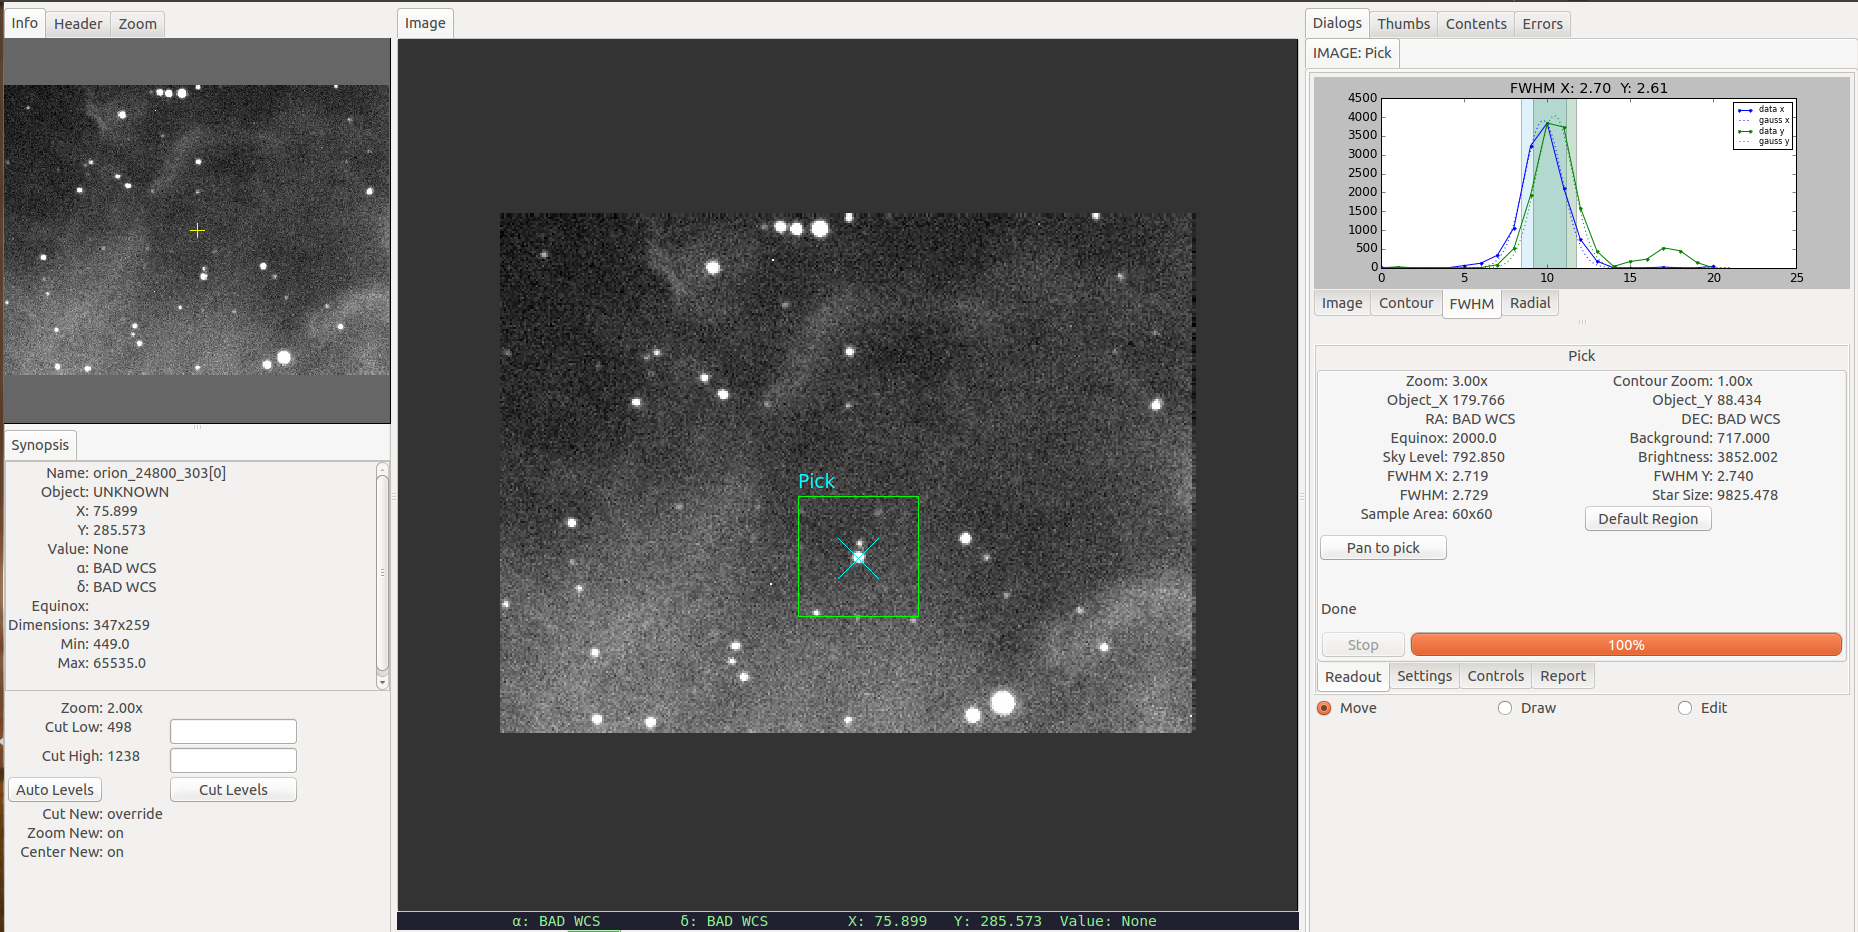
\includegraphics[width=1\linewidth]{../images/ginga}
	\caption{Ginga: Image Viewer and Toolkit}
	\label{fig:ginga}
\end{figure}

- \textbf{MaxIm DL} \cite{maximdl}, es una solución integral de análisis de imágenes astronómicas, con rutinas de enfoque automático. Es comercial, no es software libre y su precio mínimo es de 200\$.


Tras este repaso de herramientas existentes (y tras probarlas todas) tenemos una visión más o menos amplia de lo que existe en el mercado y podemos estudiar sí se pueden adaptar alguna de ellas a nuestro propósito.


Se determina que las soluciones anteriores no se adaptan exactamente a nuestro problema por diferentes causas, bien necesitan gran cantidad de software adicional para desplegarse, porque no se pueden integrar fácilmente con el driver INDI (recordemos que se encuentra implementado en Java) o son comerciales y privativas y tienen un elevado precio.


\subsection{Planificación y temporización}

Estimación de tiempos

\begin{itemize}
	\item Planteamiento del problema
	\begin{itemize}
		\item Reunión con cliente \textbf{2 horas}.
		\item Análisis inicial \textbf{5 horas}.
		\item Estudio del dominio \textbf{5 horas}.
		\item Estudio de herramientas \textbf{5 horas}.
		\item Fundamentos matemáticos curva de luz de las estrellas \textbf{8 horas}.
		\item Cálculo del FWHM \cite{fwhm} \textbf{5 horas}.
	\end{itemize}
	\item Análisis y diseño
	\begin{itemize}
		\item Diagramas \textbf{4 horas}.
		\item Diagrama algoritmo de detección \textbf{6 horas}.
	\end{itemize}
	\item Implemenantación
	\begin{itemize}
		\item Biblioteca FITS \textbf{5 horas}.
		\item Módulo de visualización \textbf{8 horas}.
		\item Resumen de la imagen \textbf{4 horas}.
		\item Algoritmos de detección de estrellas \textbf{10 horas}.
		\item Visualización de resultados gráficos \textbf{8 horas}.
		\item Visualización de resultados avanzados \textbf{5 horas}.
	\end{itemize}
	\item Pruebas \textbf{5 horas}
	\item Documentación \textbf{10 horas}

\end{itemize}

En total se estiman \textbf{95 horas} para el desarrollo de esta herramienta.   



\subsection{Análisis de requisitos}

En este punto inicial del desarrollo software, paso a identificar los requisitos funcionales y no funcionales. 
El producto final debe cumplir cada uno de ellos para adaptarse a producto que nos describe el cliente mediante entrevistas.


Señalar que la finalidad última de esta aplicación es servir como herramienta para conseguir extraer unos parámetros de ajuste de los algoritmos de enfoque, y hacer comparaciones, aunque como objetivo secundario también puede ser muy útil para visualizar imágenes FITS.


\paragraph{Requisitos funcionales}

Los requisitos funcionales nos informan de los problemas que va a tratar de solucionar el producto que estamos desarrollando.

\begin{itemize}
	\item \textbf{RF-1.}: Abrir ficheros FITS: desde un explorador de archivos debe permitir seleccionar y abrir un archivo fits.
	\item \textbf{RF-2.}: Representar los pixeles de la imagen permitiendo así una visualización de la imagen.
	
	\item \textbf{RF-3.}: Mostrar resumen de la imagen:
	\begin{itemize}
		\item \textbf{RF-3.1.}: Anchura y altura en pixeles.
		\item \textbf{RF-3.2.}: Valor del pixel más iluminado y menos iluminado.
		\item \textbf{RF-3.3.}: Media de iluminación de píxeles.
	\end{itemize} 
	
	\item \textbf{RF-4.}: Operaciones sencillas con las imágenes FITS.
	\begin{itemize}
		\item \textbf{RF-4.1.}: Hacer zoom.
		\item \textbf{RF-4.2.}: Configurar gamma.
		\item \textbf{RF-4.3.}: Configurar máximos y mínimos del histograma.
		\item \textbf{RF-4.4.}: Negativo.
	\end{itemize}
	\item \textbf{RF-5.}: Visualizar de forma gráfica la ampliación de una región de la imagen.
	\begin{itemize}
		\item \textbf{RF-5.1.}: Gráfico matricial.
		\item \textbf{RF-5.2.}: Gráfico líneas.
	\end{itemize}
	
	\item \textbf{RF-6.}:Algoritmos de detección y filtrado.
	\begin{itemize}
		\item \textbf{RF-5.1.}:  Detección de objetos.
		\item \textbf{RF-5.2.}:  Filtrado de objetos estelares.
	\end{itemize}
	
	\item \textbf{RF-7.}: Representar  resultado de los filtros de detección, coloreando las estrellas detectadas por cada uno de los filtros. 	También se debe permitir seleccionar mediante doble click los objetos interesantes.
	
	\item \textbf{RF-8.}: Resumen avanzado, con medidas como el número de objetos detectados o el valor FWHM del objeto seleccionado.
	 
\end{itemize}


\paragraph{Requisitos no funcionales}

Los requisitos no funcionales son restricciones sobre las forma de completar los requisitos funcionales propuestos. 

\begin{itemize}
	\item \textbf{RNF1.}:  Usabilidad para un usuario intermedio.
	\item \textbf{RNF2.}: Diseño modular, extensible con nuevas rutinas de detección de objetos, nuevas medidas, así como tratamiento con objetos planetarios.
	\item \textbf{RNF3.}: Eficiencia en los algoritmos de detección, para conseguir una rutina de enfoque rápida.
\end{itemize}

\subsection{Casos de uso}

Un caso de uso es una descripción de los pasos o las actividades que deber realizarse para llevar a cabo algún proceso. 
Los personajes o entidades que participarán en un caso de uso se denominan actores.

\paragraph{Descripción de actores}

\begin{itemize}
\item \textbf{Ac-1.} Usuario.
	\begin{itemize}
		\item Descripción: Persona que utiliza la aplicación.
		\item Características: Es un usuario medio/avanzado, familiarizado con la astronomía.\\
		      Desarrolladores de rutinas de enfoque y detección de objetos.
		\item Relaciones: Ninguna
		\item Atributos: Ninguno
		\item Comentarios: Ninguno.
	\end{itemize}
\end{itemize}


\paragraph{Descripción casos de uso}

\begin{itemize}
\item \textbf{CU-1.} Abrir imagen (tabla~\ref{table:cu_1}).

\begin{itemize}
	\item \textbf{Actores:} Usuario.
	\item \textbf{Tipo:} Primario, esencial.
	\item \textbf{Referencias:} 
	\item \textbf{Precondición:}
	\item \textbf{Postcondición:} El sistema carga un archivo de imagen y se visualiza en la pantalla principal.
	\item \textbf{Autor:} José Miguel López.
	\item \textbf{Versión:} 1.0.
	\item \textbf{Propósito:} Introducir en el sistema un fichero de imagen.
	\item \textbf{Resumen:} El usuario selecciona un archivo de imagen del sistema de ficheros de la computadora,  al aceptar el sistema carga la imagen y se visualiza. 
\end{itemize}
		   
\begin{table}[!ht]
	\begin{center}
		\begin{tabular}{|l|l|l|l|}
			\hline
			\multicolumn{4}{|c|}{{\bf Curso normal}}
			\\ \hline
			\multicolumn{2}{|c|}{{\bf Actor}} & \multicolumn{2}{c|}{{\bf Sistema}}
			\\ \hline
			{\it 1} & 
			\begin{tabular}[c]{@{}l@{}}
				Usuario: Pulsa el botón para\\
				abrir una imagen.\\
			\end{tabular} &
			&
			\\ \hline
			&
			&
			{\it 2} &
			\begin{tabular}[c]{@{}l@{}}
				El sistema muestra un explorador \\
				con los ficheros y directorios de la máquina. \\
			\end{tabular}
			\\ \hline
			{\it 3} & 
			\begin{tabular}[c]{@{}l@{}}
				Usuario: Selecciona un archivo \\
				con formato \textbf{fits} y pulsa en el \\
				botón de aceptar.   \\
			\end{tabular} &
			&
			\\ \hline
			&
			&
			{\it 4} &
			\begin{tabular}[c]{@{}l@{}}
				Se visualiza la imagen en pantalla \\
				Se muestra  resumen de la imagen\\
				Anchura, altura, valor píxel más oscuro \\
				valor píxel más iluminado, \\
				media luminosidad de los píxeles.\\
			\end{tabular}
			\\ \hline
		\end{tabular}
		\caption{CU-1. Abrir imagen FITS.}
		\label{table:cu_1}
	\end{center}
\end{table}



\item \textbf{CU-2.} Modificar gamma (tabla~\ref{table:cu_2}).
\begin{itemize}
	\item\textbf{ Actores:} Usuario.
	\item \textbf{Tipo:} Primario, esencial.
	\item \textbf{Referencias}: 
	\item \textbf{Precondición:} El usuario has de haber completado el CU-1
	\item \textbf{Postcondición:} Se actualiza la imagen con la nueva configuración de gamma.
	\item \textbf{Autor:} José Miguel López.
	\item \textbf{Versión:} 1.0.
	\item \textbf{Propósito:} Modificar visualización de la imagen.
	\item \textbf{Resumen:} El usuario modificar el valor del campo gamma. Para entender bien el efecto consultar la referencia Gamma \cite{gamma}.
\end{itemize}


\begin{table}[!ht]
	\begin{center}
		\begin{tabular}{|l|l|l|l|}
			\hline
			\multicolumn{4}{|c|}{{\bf Curso normal}}
			\\ \hline
			\multicolumn{2}{|c|}{{\bf Actor}} & \multicolumn{2}{c|}{{\bf Sistema}}
			\\ \hline
			{\it 1} & 
			\begin{tabular}[c]{@{}l@{}}
				Usuario: Selecciona un valor \\
				de compensación de gamma\\
				entre 0.05 y 10 \\
			\end{tabular} &
			&
			\\ \hline
			&
			&
			{\it 2} &
			\begin{tabular}[c]{@{}l@{}}
				El sistema computa \\
				el valor de los píxeles \\
				y muestra la imagen con la corrección \\
				de gamma aplicada \\ 
			\end{tabular}
			\\ \hline
		\end{tabular}
		\caption{CU-2. Modificar Gamma.}
		\label{table:cu_2}
	\end{center}
\end{table}


\item \textbf{CU-3.} Modificar ecuación del histograma (tabla~\ref{table:cu_3}).
	\begin{itemize}
		\item \textbf{Actores:} Usuario.
		\item \textbf{Tipo:} Primario, esencial.
		\item \textbf{Referencias:} 
		\item \textbf{Precondición:} El usuario has de haber completado el CU-1
		\item \textbf{Postcondición:} Se actualiza la imagen con la nueva configuración del histograma.
		\item \textbf{Autor:} José Miguel López.
		\item \textbf{Versión:} 1.0.
		\item \textbf{Propósito:} Modificar visualización de la imagen.
		\item \textbf{Resumen:} El usuario modificar el valor mínimo o máximo del histograma.
	\end{itemize}
	
\begin{table}[!ht]
	\begin{center}
		\begin{tabular}{|l|l|l|l|}
			\hline
			\multicolumn{4}{|c|}{{\bf Curso normal}}
			\\ \hline
			\multicolumn{2}{|c|}{{\bf Actor}} & \multicolumn{2}{c|}{{\bf Sistema}}
			\\ \hline
			{\it 1} & 
			\begin{tabular}[c]{@{}l@{}}
				Usuario: Selecciona un valor \\
				de min y max entre el 0 \\
				y el valor del píxel más luminoso \\
			\end{tabular} &
			&
			\\ \hline
			&
			&
			{\it 2} &
			\begin{tabular}[c]{@{}l@{}}
				El sistema muestra la imagen \\
				 según una nueva ecuación de histograma,\\
				 ello repercute en el brillo y contraste. \\ 
			\end{tabular}
			\\ \hline
		\end{tabular}
		\caption{CU-3.Modificar ecuación Histograma de la Imagen.}
		\label{table:cu_3}
	\end{center}
\end{table}
	
	


\item \textbf{CU-4.} Modificar zoom (tabla~\ref{table:cu_4}).
	\begin{itemize}
		\item \textbf{Actores:} Usuario.
		\item \textbf{Tipo:} Primario, esencial.
		\item \textbf{Referencias:} 
		\item \textbf{Precondición:} El usuario has de haber completado el CU-1
		\item \textbf{Postcondición:} Se amplia o reduce la visualización de la imagen.
		\item \textbf{Autor:} José Miguel López.
		\item \textbf{Versión:} 1.0.
		\item \textbf{Propósito:} Ampliar o reducir la visualización de la imagen.
		\item  \textbf{Resumen:} El usuario modificar el valor zoom y la imagen se amplia o reduce.
\end{itemize}

\begin{table}[!ht]
	\begin{center}
		\begin{tabular}{|l|l|l|l|}
			\hline
			\multicolumn{4}{|c|}{{\bf Curso normal}}
			\\ \hline
			\multicolumn{2}{|c|}{{\bf Actor}} & \multicolumn{2}{c|}{{\bf Sistema}}
			\\ \hline
			{\it 1} & 
			\begin{tabular}[c]{@{}l@{}}
				Usuario: Selecciona un valor \\
				de zoom entre el   25\%  y el  100\%  \\
			\end{tabular} &
			&
			\\ \hline
			&
			&
			{\it 2} &
			\begin{tabular}[c]{@{}l@{}}
				El sistema muestra la imagen \\
				con el nuevo escalado \\ 
			\end{tabular}
			\\ \hline
		\end{tabular}
		\caption{CU-4.Modificar Zoom.}
		\label{table:cu_4}
	\end{center}
\end{table}


\item \textbf{CU-5}. Generar gráfico de zona (tabla~\ref{table:cu_5}).
\begin{itemize}


\item \textbf{Actores:} Usuario.
\item \textbf{Tipo:} Primario, esencial.
\item \textbf{Referencias:} 
\item \textbf{Precondición:} El usuario has de haber completado el CU-1 y hace click en una zona de la imagen.
\item \textbf{Postcondición:} Genera un gráfico en forma matriz (mapa de calor) y líneas con una ampliación de una zona de la imagen.
\item \textbf{Autor:} José Miguel López.
\item \textbf{Versión:} 1.0.
\item \textbf{Propósito:} Generar gráfico de detalle de una zona.
\item \textbf{Resumen:} El usuario hace click en una zona de la imagen y se muestran gráficos de luz de la zona con tales coordenadas.
\end{itemize}

\begin{table}[!ht]
	\begin{center}
		\begin{tabular}{|l|l|l|l|}
			\hline
			\multicolumn{4}{|c|}{{\bf Curso normal}}
			\\ \hline
			\multicolumn{2}{|c|}{{\bf Actor}} & \multicolumn{2}{c|}{{\bf Sistema}}
			\\ \hline
			{\it 1} & 
			\begin{tabular}[c]{@{}l@{}}
				Usuario: Hace click en un punto \\
				de la imagen.  \\
			\end{tabular} &
			&
			\\ \hline
			&
			&
			{\it 2} &
			\begin{tabular}[c]{@{}l@{}}
				El sistema genera un gráfico de luz \\
				del entorno del punto seleccionado. \\
			\end{tabular}
			\\ \hline
		\end{tabular}
		\caption{CU-5.Generar Gráfico luz de zona.}
		\label{table:cu_5}
	\end{center}
\end{table}



\begin{itemize}


\item \textbf{CU-6.} Activar detección de objetos (tabla~\ref{table:cu_6}).
	\begin{itemize}
		\item \textbf{Actores:} Usuario.
		\item \textbf{Tipo:} Primario, esencial.
		\item \textbf{Referencias:} 
		\item \textbf{Precondición:} El usuario has de haber completado el CU-1.
		\item \textbf{Postcondición:} Se hace una búsqueda inicial de objetos, siguiendo el algoritmos de máximo locales y marcan con puntos de color.
		\item \textbf{Autor:} José Miguel López.
		\item \textbf{Versión:} 1.0.
		\item \textbf{Propósito:} Hacer una búsqueda inicial de objetos estelares.
		\item \textbf{Resumen:} El usuario activa la casilla de detección de objetos, y se pintan en pantalla puntos donde pueden existir objetos.
	\end{itemize}
\end{itemize}

\begin{table}[!ht]
	\begin{center}
		\begin{tabular}{|l|l|l|l|}
			\hline
			\multicolumn{4}{|c|}{{\bf Curso normal}}
			\\ \hline
			\multicolumn{2}{|c|}{{\bf Actor}} & \multicolumn{2}{c|}{{\bf Sistema}}
			\\ \hline
			{\it 1} & 
			\begin{tabular}[c]{@{}l@{}}
				Usuario: Activa función ``Detect Stars`` y \\
				establece valor \\
				``Radius surrounding peak`` \\
				entre 1 y 20. \\
			\end{tabular} &
			&
			\\ \hline
			&
			&
			{\it 2} &
			\begin{tabular}[c]{@{}l@{}}
				El sistema busca objetos estelares \\
				que respondan a un pico de luz\\ en el radio 
				seleccionado. \\
				Los objetos detectados son \\ marcados en color. 
			\end{tabular}
			\\ \hline
		\end{tabular}
		\caption{CU-6. Activar detección de objetos..}
		\label{table:cu_6}
	\end{center}
\end{table}




\item \textbf{CU-7.} Generar gráfico de objeto (tabla~\ref{table:cu_7}).
	\begin{itemize}
		\item Actores: Usuario.
		\item Tipo: Primario, esencial.
		\item Referencias: 
		\item Precondición: El usuario has de haber completado el CU-1  y el CU-5
		\item Postcondición: Genera un gráfico en forma matriz (mapa de calor) y líneas con una ampliación del objeto.
		\item Autor: José Miguel López.
		\item Versión: 1.0.
		\item Propósito: Generar gráficos de detalle del objeto 
		\item Resumen: El usuario hace doble click en un objeto y se muestran gráficos de luz del objeto. 
	\end{itemize}

\begin{table}[!ht]
	\begin{center}
		\begin{tabular}{|l|l|l|l|}
			\hline
			\multicolumn{4}{|c|}{{\bf Curso normal}}
			\\ \hline
			\multicolumn{2}{|c|}{{\bf Actor}} & \multicolumn{2}{c|}{{\bf Sistema}}
			\\ \hline
			{\it 1} & 
			\begin{tabular}[c]{@{}l@{}}
				Usuario: Hace doble clic \\
				en un objeto detectado.  \\
			\end{tabular} &
			&
			\\ \hline
			&
			&
			{\it 2} &
			\begin{tabular}[c]{@{}l@{}}
				El sistema genera un gráfico de luz \\
				del entorno al objeto seleccionado. \\
			\end{tabular}
			\\ \hline
		\end{tabular}
		\caption{CU-7. Generar Gráfico luz de objeto.}
		\label{table:cu_7}
	\end{center}
\end{table}



\item \textbf{CU-8.} Aplicar filtro margen (tabla~\ref{table:cu_8}).
	\begin{itemize}
		\item Actores: Usuario.
		\item Tipo: Primario, esencial.
		\item Referencias: 
		\item Precondición: El usuario has de haber completado el CU-1  y el CU-5
		\item Postcondición: Se descartan los objetos situados a una distancia del borde de la imagen.
		\item Autor: José Miguel López.
		\item Versión: 1.0.
		\item Propósito: Descartar objetos cerca del borde de la imagen.
		\item Resumen:  
	\end{itemize}

\begin{table}[!ht]
	\begin{center}
		\begin{tabular}{|l|l|l|l|}
			\hline
			\multicolumn{4}{|c|}{{\bf Curso normal}}
			\\ \hline
			\multicolumn{2}{|c|}{{\bf Actor}} & \multicolumn{2}{c|}{{\bf Sistema}}
			\\ \hline
			{\it 1} & 
			\begin{tabular}[c]{@{}l@{}}
				Usuario: Marca la casilla \\
				``Filter Margin Stars`` \\
				y establece un valor \\
				``Margin Size`` entre 1 y 40. \\
			\end{tabular} &
			&
			\\ \hline
			&
			&
			{\it 2} &
			\begin{tabular}[c]{@{}l@{}}
				El sistema marca las estrellas a distancia \\
				``Margin Size `` píxeles como descartadas. \\
			\end{tabular}
			\\ \hline
		\end{tabular}
		\caption{CU-8.Aplicar filtro margen.}
		\label{table:cu_8}
	\end{center}
\end{table}


\item \textbf{CU-9.} Aplicar filtro contraste (tabla~\ref{table:cu_9}).
	\begin{itemize}
		\item Actores: Usuario.
		\item Tipo: Primario, esencial.
		\item Referencias: 
		\item Precondición: El usuario has de haber completado el CU-1  y el CU-5
		\item Postcondición: Se descartan objetos estelares que no cumplan con un perfil de contraste dado.
		\item Autor: José Miguel López.
		\item Versión: 1.0.
		\item Propósito: Eliminar objetos que no cumplan un perfil de contraste dado, descartando así falsos positivos en la detección inicial.
		\item Resumen:  
	\end{itemize}

\begin{table}[!ht]
	\begin{center}
		\begin{tabular}{|l|l|l|l|}
			\hline
			\multicolumn{4}{|c|}{{\bf Curso normal}}
			\\ \hline
			\multicolumn{2}{|c|}{{\bf Actor}} & \multicolumn{2}{c|}{{\bf Sistema}}
			\\ \hline
			{\it 1} & 
			\begin{tabular}[c]{@{}l@{}}
				Usuario: Marca la casilla \\
				``Contrast Filter`` \\
				y establece un valor para \\
				``Radius`` entre 1 y 20 y \\
				``Minimun Quotient`` entre 1 y 10. \\
			\end{tabular} &
			&
			\\ \hline
			&
			&
			{\it 2} &
			\begin{tabular}[c]{@{}l@{}}
				El sistema marca las estrellas \\ 
				que no responda al perfil de contraste,\\
				 como rechazas \\
				 (Cociente entre punto más luminosos \\
				  del objeto y mínimo del entorno)\\
				 
			\end{tabular}
			\\ \hline
		\end{tabular}
		\caption{CU-9.Aplicar filtro contraste.}
		\label{table:cu_9}
	\end{center}
\end{table}





\item \textbf{CU-10.} Aplicar filtro distancia entre objetos (tabla~\ref{table:cu_10}).
	\begin{itemize}
		\item Actores: Usuario.
		\item Tipo: Primario, esencial.
		\item Referencias: 
		\item Precondición: El usuario has de haber completado el CU-1  y el CU-5
		\item Postcondición: Se descartan objetos que estén próximos los unos a los otros.
		\item Autor: José Miguel López.
		\item Versión: 1.0.
		\item Propósito: Eliminar objetos que se encuentren muy próximos entre ellos.
		\item Resumen:  
	\end{itemize}


\begin{table}[!ht]
	\begin{center}
		\begin{tabular}{|l|l|l|l|}
			\hline
			\multicolumn{4}{|c|}{{\bf Curso normal}}
			\\ \hline
			\multicolumn{2}{|c|}{{\bf Actor}} & \multicolumn{2}{c|}{{\bf Sistema}}
			\\ \hline
			{\it 1} & 
			\begin{tabular}[c]{@{}l@{}}
				Usuario: Marca la casilla \\
				``Distance Filter`` \\
				y establece un valor para \\
				``Distance`` entre 1 y 500 \\
			\end{tabular} &
			&
			\\ \hline
			&
			&
			{\it 2} &
			\begin{tabular}[c]{@{}l@{}}
				El sistema marca las estrellas  \\
				 próximas unas a otras a una distancia \\ 
				 inferior a ``Distance`` \\
				 como rechazadas. \\
			\end{tabular}
			\\ \hline
		\end{tabular}
		\caption{CU-10.Aplicar filtro distancia.}
		\label{table:cu_10}
	\end{center}
\end{table}



\item \textbf{CU-11.} Aplicar filtro FWHM (tabla~\ref{table:cu_11}).
	\begin{itemize}
		\item Actores: Usuario.
		\item Tipo: Primario, esencial.
		\item Referencias: 
		\item Precondición: El usuario has de haber completado el CU-1  y el CU-5.
		\item Postcondición: Se descartan objetos que no respondan a un perfil FWHM dado.
		\item Autor: José Miguel López.
		\item Versión: 1.0.
		\item Propósito: Eliminar objetos que no respondan a un perfil \textbf{FWHM}.
		\item Resumen:  
	\end{itemize}



\begin{table}[!ht]
	\begin{center}
		\begin{tabular}{|l|l|l|l|}
			\hline
			\multicolumn{4}{|c|}{{\bf Curso normal}}
			\\ \hline
			\multicolumn{2}{|c|}{{\bf Actor}} & \multicolumn{2}{c|}{{\bf Sistema}}
			\\ \hline
			{\it 1} & 
			\begin{tabular}[c]{@{}l@{}}
				Usuario: Marca la casilla \\
				``FWHM Filter`` \\
				y establece un valor para \\
				``Minimun value`` entre 1 y 40 y \\
				``Radius`` entre 1 y 100. \\
			\end{tabular} &
			&
			\\ \hline
			&
			&
			{\it 2} &
			\begin{tabular}[c]{@{}l@{}}
				El sistema marca las estrellas  \\
				que no respondan al perfil FWHM \\
				como rechazadas. \\
			\end{tabular}
			\\ \hline
		\end{tabular}
		\caption{CU-11.Aplicar filtro FWHM.}
		\label{table:cu_11}
	\end{center}
\end{table}



\item \textbf{CU-12.} Aplicar número de objetos (tabla~\ref{table:cu_12}).
	\begin{itemize}
		\item Actores: Usuario.
		\item Tipo: Primario, esencial.
		\item Referencias: 
		\item Precondición: El usuario has de haber completado el CU-1  y el CU-5 
		\item Postcondición: Se descargan todos los objetos menos los más luminosos.
		\item Autor: José Miguel López.
		\item Versión: 1.0.
		\item Propósito: Descartar los objetos menos luminosos de la imagen.
		\item Resumen:  
	\end{itemize}


\begin{table}[!ht]
	\begin{center}
		\begin{tabular}{|l|l|l|l|}
			\hline
			\multicolumn{4}{|c|}{{\bf Curso normal}}
			\\ \hline
			\multicolumn{2}{|c|}{{\bf Actor}} & \multicolumn{2}{c|}{{\bf Sistema}}
			\\ \hline
			{\it 1} & 
			\begin{tabular}[c]{@{}l@{}}
				Usuario: Marca la casilla \\
				``Number Filter`` \\
				 y establece un valor para \\
				``Number Star``.
			\end{tabular} &
			&
			\\ \hline
			&
			&
			{\it 2} &
			\begin{tabular}[c]{@{}l@{}}
				El sistema marca las X ``Number Star``\\
				estrellas como válidas y descarta el resto.  \\
			\end{tabular}
			\\ \hline
		\end{tabular}
		\caption{CU-12.Aplicar número de objetos.}
		\label{table:cu_12}
	\end{center}
\end{table}



\item \textbf{CU-13.} Aplicar filtro ajuste Gauss (tabla~\ref{table:cu_13}).
	\begin{itemize}
		\item Actores: Usuario.
		\item Tipo: Primario, esencial.
		\item Referencias: 
		\item Precondición: El usuario has de haber completado el CU-1  y el CU-5
		\item Postcondición:Se descartan los objetos cuya curva de luz no responda a una curva de Gauss con los parámetros dados. \\
		\item Autor: José Miguel López.
		\item Versión: 1.0.
		\item Propósito: Descartar objetos que no respondan a una curva de Gauss dada por parámetros.
		\item Resumen:  
	\end{itemize}



\begin{table}[!ht]
	\begin{center}
		\begin{tabular}{|l|l|l|l|}
			\hline
			\multicolumn{4}{|c|}{{\bf Curso normal}}
			\\ \hline
			\multicolumn{2}{|c|}{{\bf Actor}} & \multicolumn{2}{c|}{{\bf Sistema}}
			\\ \hline
			{\it 1} & 
			\begin{tabular}[c]{@{}l@{}}
				Usuario: Marca la casilla \\
				``Gaussian Filter`` \\
				y establece un valor para \\
				``Radius``, ``Normal``, ``Mean`` y ``Sigma``.
			\end{tabular} &
			&
			\\ \hline
			&
			&
			{\it 2} &
			\begin{tabular}[c]{@{}l@{}}
				El sistema marca las estrellas \\
				que no respondan cuyo curva de luz \\
				no responda a una curva de Gauss \\
			\end{tabular}
			\\ \hline
		\end{tabular}
		\caption{CU-13. Aplicar filtro ajuste Gauss..}
		\label{table:cu_13}
	\end{center}
\end{table}


\end{itemize}




\subsection{Diagrama de casos de uso}

Los diagramas de casos de uso sirven para representar los relaciones que existen entre los diferentes actores y el sistema. Dado que en nuestro caso solo hay un actor, todos los casos de uso son iniciados por él (figura~\ref{fig:casos_uso}).

\begin{figure}[!ht]
\centering
\includegraphics[width=0.7\linewidth]{../images/casos_uso}
\caption{Diagrama de casos de uso.}
\label{fig:casos_uso}
\end{figure}




\section{Diseño e implementación}

El diseño de la aplicación puede dividirse en las siguientes partes:


\begin{itemize}
	\item \textbf{Diseño de clases.}
	\item \textbf{Diseño de algoritmos de detección.}
	\item \textbf{Diseño de interfaz de usuario.}
\end{itemize}


\subsection{Diseño de clases}

El diseño de las clases define la arquitectura de la aplicación. Llevar a cabo una buena arquitectura determina la calidad, facilidad ante cambios o ampliaciones futuras, así como la propia implementación, testeo y corrección de posibles errores. En la figura~\ref{fig:diagrama_clases} se muestra un pequeño diagrama de clases de la aplicación.


\begin{figure}
\centering
\includegraphics[width=1\linewidth]{../images/diagrama_clases}
\caption{Diagrama de clases}
\label{fig:diagrama_clases}
\end{figure}


Las clases principales con las que cuenta nuestra aplicación son las siguientes:


\begin{itemize}
	\item \texttt{FitsImage}: Realiza una abstracción de las propiedades  y operaciones con las imágenes.
	
	
	Las imágenes se encuentran en formato FITS. Para poder trabajar con ellas desde Java hacemos uso de la biblioteca \texttt{jfits} \cite{jfits}. Con ella tenemos acceso a los datos (píxeles de la matriz), y a los metadatos que que incorporan la cabecera. 
	
	
	Para facilitar la programación se implementa una clase que encapsula los atributos y métodos para manejar imágenes FITS: \texttt{FitsImage}.
	
	\item \texttt{Star}: Realiza una abstración de las propiedades  y operaciones con los objetos estelares (estrellas). 
	\item \texttt{Processing}: Encapsula funciones y operaciones avanzadas de procesamiento y búsqueda de objetos.
	\item \texttt{Utils}: Operaciones de uso común en la aplicación, principalmente manejo de matrices y matemáticas. 
\end{itemize}


\subsection{Diseño de interfaz de usuario}

En la figura~\ref{fig:mockuppp} se muestra un \textbf{mockup} aproximado donde se puede ver como ser organizan visualmente los elementos dentro de la interfaz de la aplicación.

\begin{figure}[!ht]
	\centering
	\includegraphics[width=1\linewidth]{../images/mockup}
	\caption{Mockup interfaz}
	\label{fig:mockuppp}
\end{figure}


En la figura~\ref{fig:start_pocesor} se muestra el aspecto de la aplicación terminada.

\begin{figure}
\centering
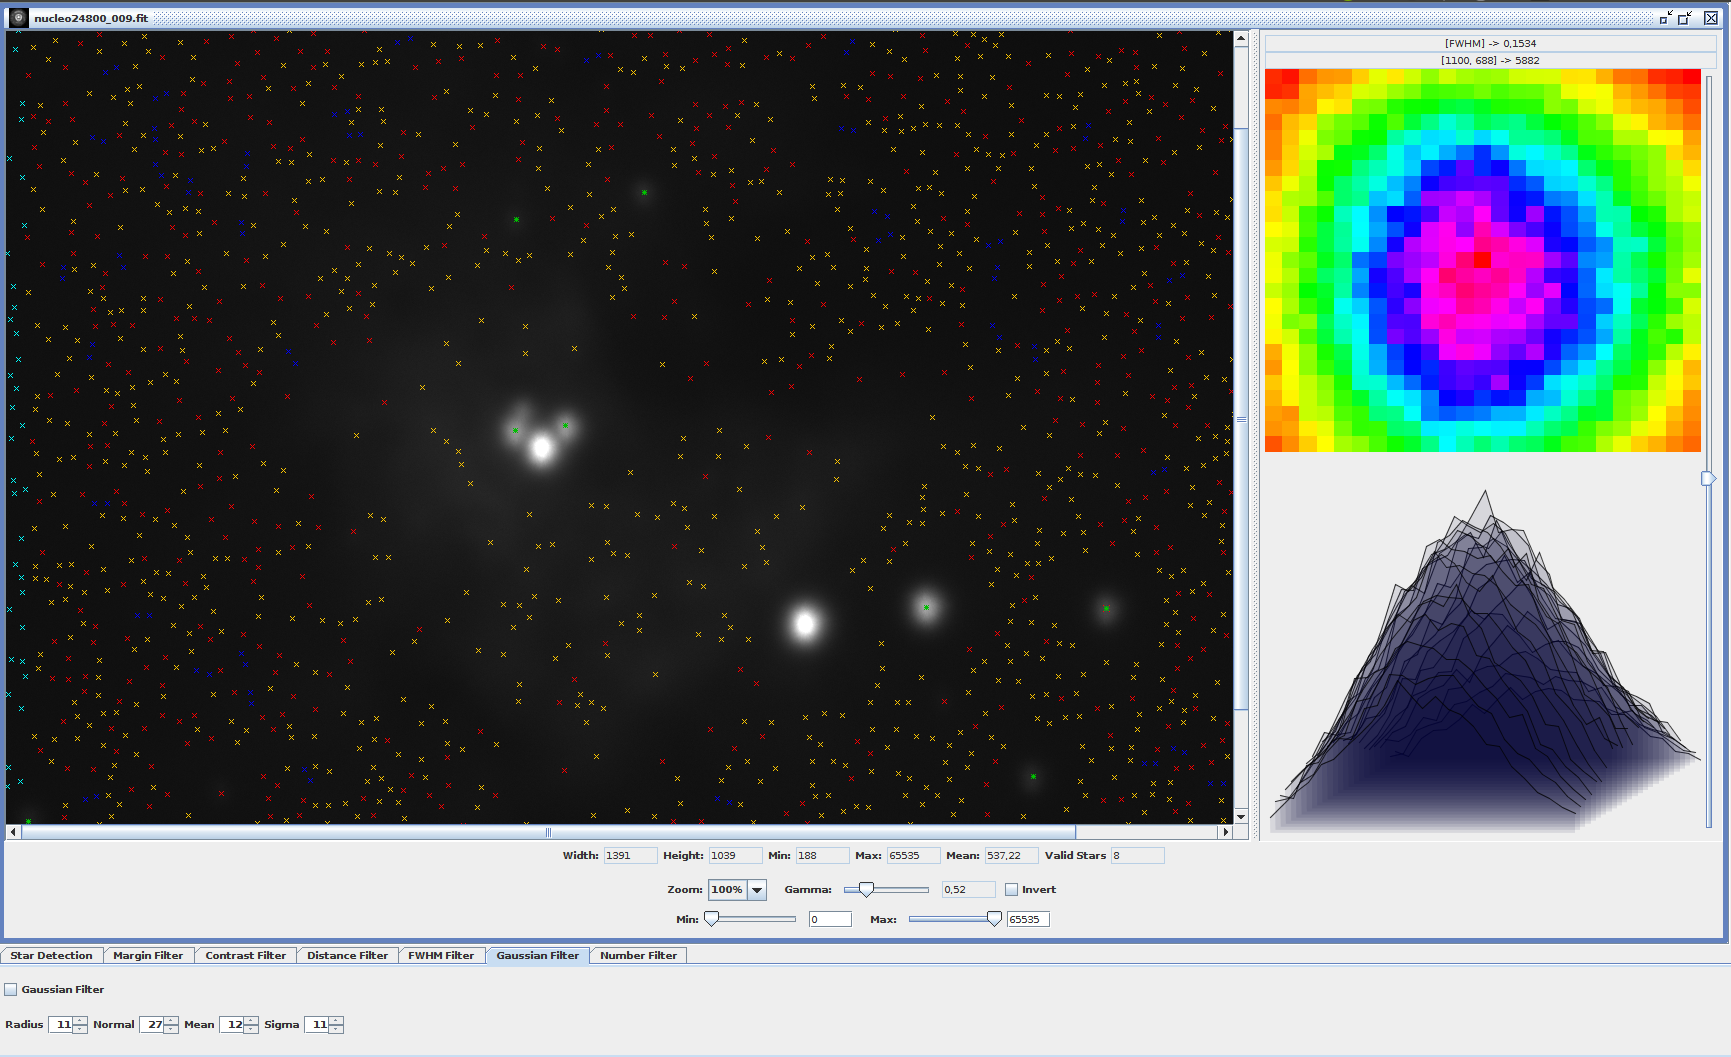
\includegraphics[width=1\linewidth]{../images/start_pocesor}
\caption{Aplicación Star Focusing}
\label{fig:start_pocesor}
\end{figure}

\section{Algoritmos de detección}

Las imágenes que analizamos cuentan con gran cantidad de objetos estelares, que debemos ser capaces de detectar y filtrar según los patrones que nos interesen. El objetivo de aplicar detección de objetos es poder detectar la posición de los objetos e la imagen que queremos enfocar: en este caso, estrellas (figura~\ref{fig:estrella}).

\begin{figure}
	\centering
	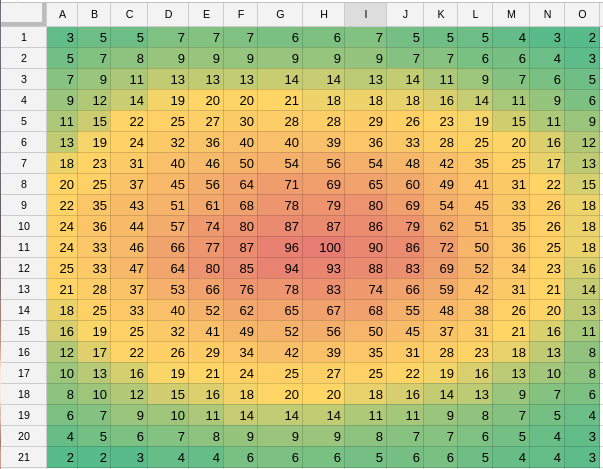
\includegraphics[width=0.8\linewidth]{../images/estrella}
	\caption{Mapa de calor de una estrella}
	\label{fig:estrella}
\end{figure}

Para la detección de objetos utilizamos las siguientes rutinas:

\begin{enumerate}
	\item Algoritmo búsqueda máximo local absolutos, tomando en cuenta puntos máximos en la imagen. Detecta falsos positivos, así como píxeles calientes aislados.  
	
	\item Región de puntos con tendencia descendente. Consiste en detectar regiones donde exista una sucesión de radio \texttt{x}, cuyo valor siga una tendencia clara, esta solución es bastante mejor aproximación que la anterior y elimina el problema de los píxeles calientes. No es óptimo pero se puede usar como un filtro de grano grueso.
\end{enumerate}





Para considerar que un objeto es una estrella es condición necesaria, pero no suficiente que cumpla lo anterior.

Para asegurarnos de que realmente hemos encontrado un objeto estelar debemos aplicar una serie de filtros adicionales al resultado anterior y eliminar progresivamente falsos positivos, así como casos poco interesantes. 

\begin{enumerate}
	\item Filtro por perfil de contraste, resultado de dividir los valores altos y valores bajos, tiene un cociente alto. Esto indica que es esa región de la imagen existe una perturbación importante de luz. Dado que con el algoritmo anterior ya tenemos un conjunto de candidatos, se puede hacer de forma eficiente solo sobre los puntos previamente encontrados. 
	
	\item Filtro gaussiano y FWHM. Consisten en buscar regiones de la imagen donde se de un ajuste de la gaussiana dentro de cierto parámetros, la normal, el sigma o directamente calcular el FWHM. Este proceso es costoso y pesado, por tanto se debe aplicar a un conjunto muy pequeño de regiones, que previamente hayan pasado los filtros anteriores.
	
	El perfil de cada estrella se puede aproximar con una curva Gaussiana, asumiendo que cuanto mejor el ajuste a tal curva, mejor es el enfoque obtenido en la imagen.
	
	El perfil  de dicha gaussiana se caracteriza por su ancho en la mitad de su valor máximo o \textbf{FWHM} (Full Width at Half Maximum \cite{fwhm}), este valor solo sé ve afectado por el seeing \cite{seeing}, o la distorsión de la atmósfera, siendo constante para todos los objetos estelares en una misma imagen. FWHM, es una medida del efecto provocado por la dispersión del haz de luz que provoca que las estrellas no aparezcan como puntos sino como discos.
		
	\item  Filtros adicionales. Podemos eliminar objetos cuyo máximo este por encima o por debajo de cierto valor.
	Estrellas muy cercanas entre sí o estrellas próximas a los límites de la imagen. 	
\end{enumerate}

Todo estas rutinas de filtrado quedan encapsuladas en la clase \texttt{Processing}.


\section{Evaluación nivel de enfoque}

Una vez detectadas las estrellas, debemos determinar una medida para evaluar las calidad del enfoque.

El perfil en la imagen de cada estrella se puede aproximar con una curva Gaussiana 2D (figura~\ref{fig:estrellaGauss}).


\begin{figure}
	\centering
	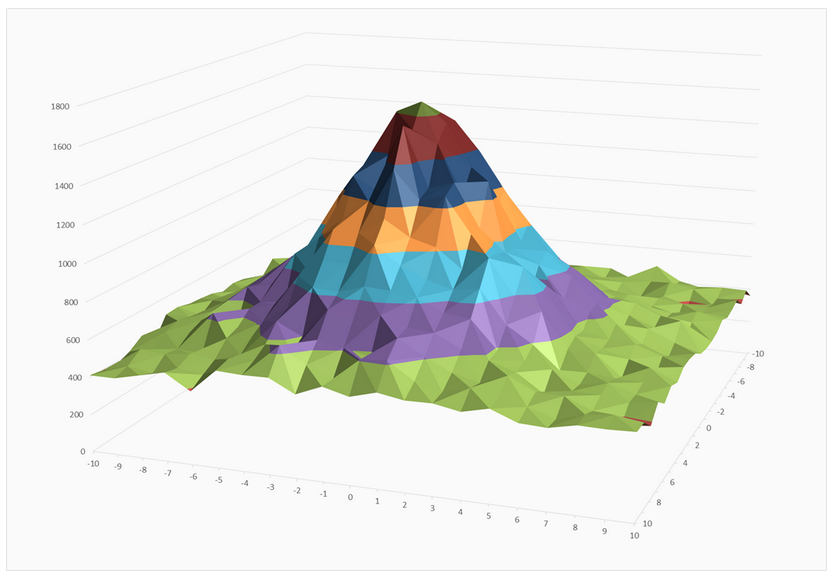
\includegraphics[width=0.9\linewidth]{../images/estrella_gauss}
	\caption{Ajuste Gaussiana de una Estrella}
	\label{fig:estrellaGauss}
\end{figure}


Una característica de la curva de Gauss que nos da información de la calidad del enfoque de un objeto es la medida FWHM (Full width at half maximum, ancho total a mital del máximo [figura~\ref{fig:FWHM}]).


Cuando la función considerada es una distribución normal de la forma: 


	$$ f(x) = \frac{1}{\sigma \sqrt{2 \pi} } \exp \left[ -\frac{(x-x_0)^2}{2 \sigma^2} \right] $$

Donde  $ \sigma $ es la desviación típica y  $x_0$ puede ser cualquier valor (la anchura de la función no cambia con una traslación). La relación entre FWHM y la desviación típica es \cite{wolfram}: 

$$  \mathrm{FWHM} =   2 \sqrt{2 \ln 2 } \; \sigma \approx 2.35482 \; \sigma $$

	\begin{figure}[h]
		\centering
		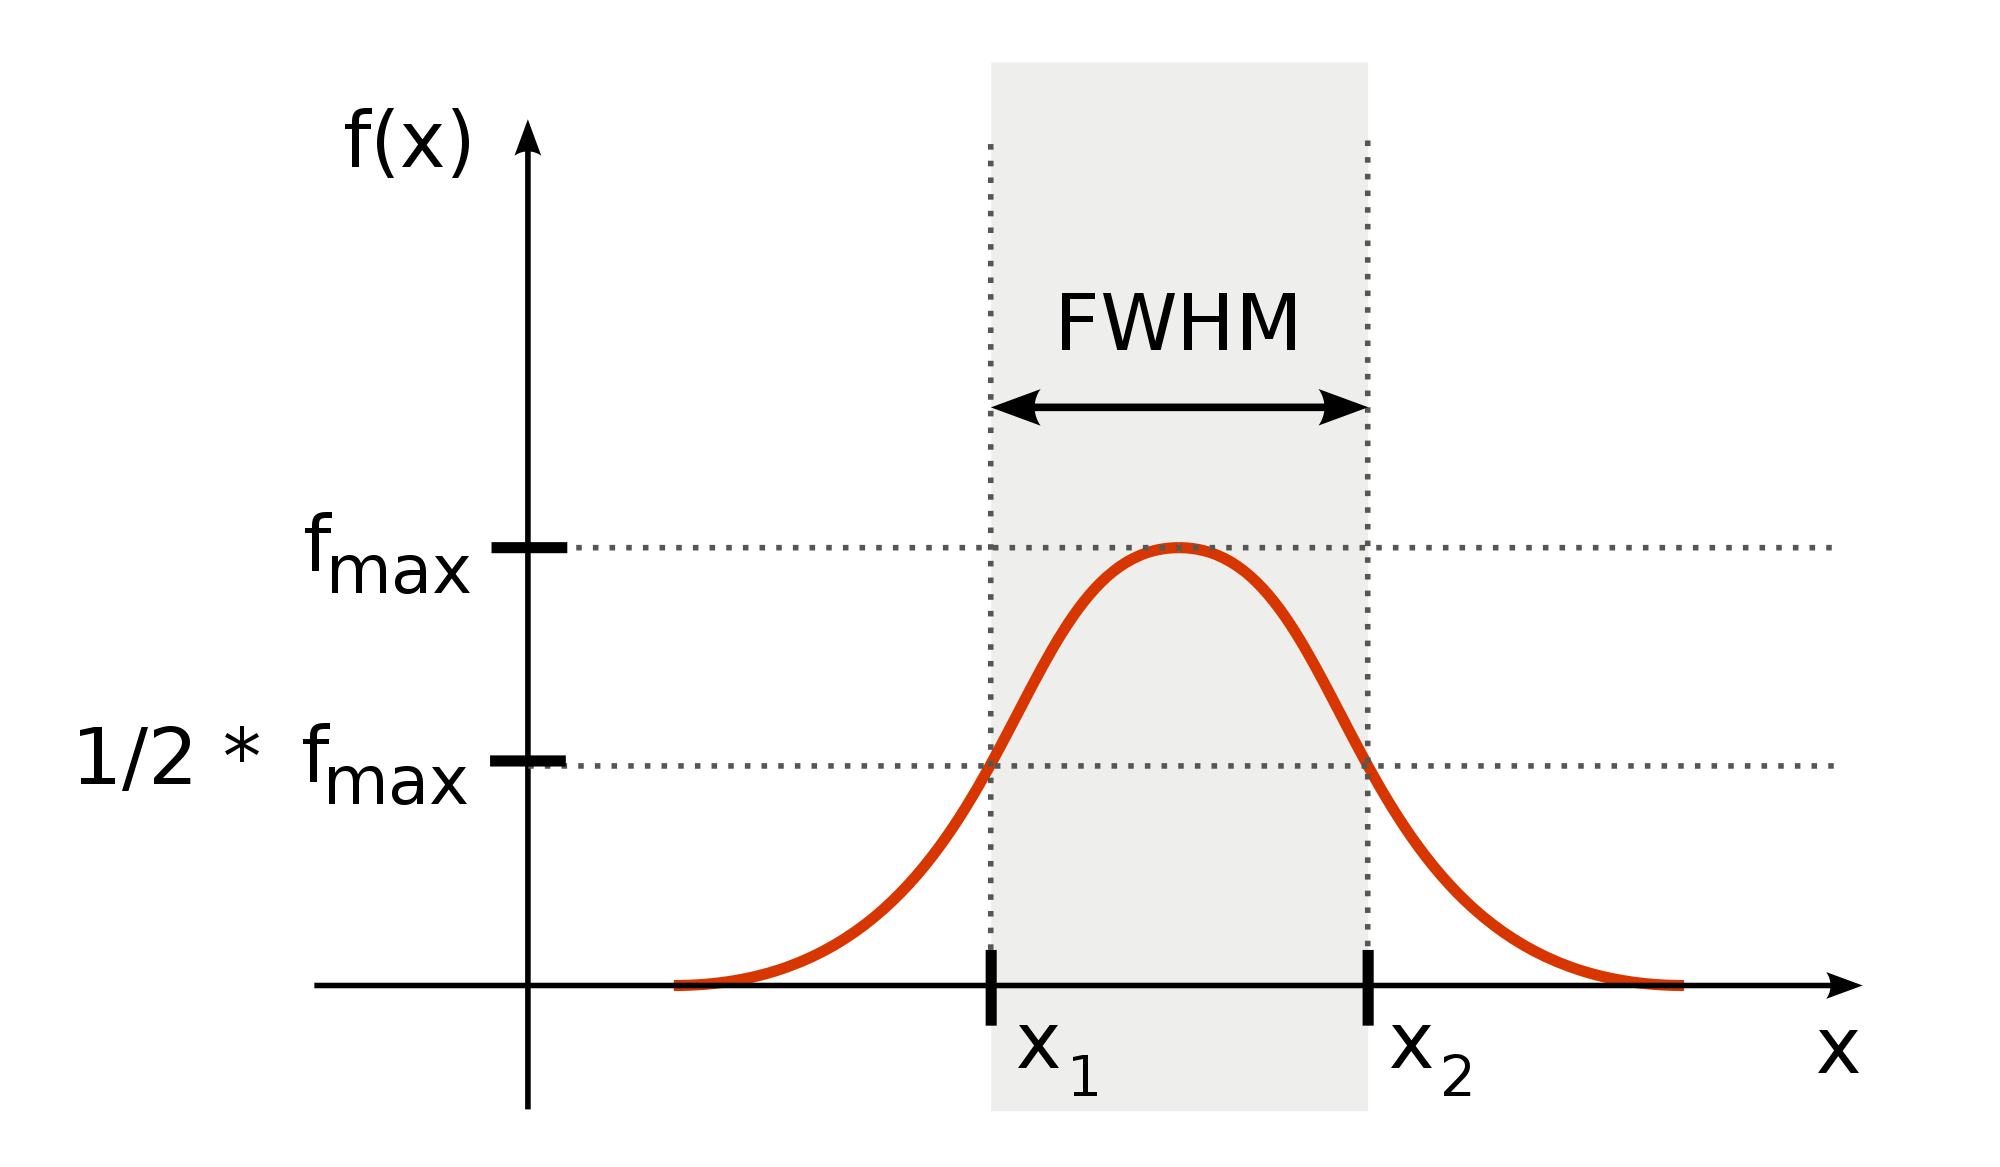
\includegraphics[width=0.7\linewidth]{../images/FWHM}
		\caption[Grafica FWHM]{Gráfica FWHM. \textbf{Fuente:} \cite{fwhm}}
		\label{fig:FWHM}
	\end{figure}


El FWHM puede medirse en diferentes ejes (en el eje X y en el eje Y por ejemplo).
Si las estrellas son redondas, como comentábamos en el apartado anterior, el FWHM debe ser el mismo en cualquier eje.
La diferencia entre los ejes X e Y puede utilizarse como medida de la redondez de la estrella.


\textbf{Pasos para el cálculo del FWHM:}
\begin{itemize}
	\item \textbf{Ajustar perfil de luz a una Gausiana.}
	
	Se implementa el método \texttt{computeGaussianParams}
	
	Que recibe como parámetros:
	
	\begin{itemize}
		\item Matriz de pixeles de la imagen.
		\item Coordenadas punto central del objeto.
		\item Radio del objeto o zona. 
	\end{itemize} 
	
	Haciendo uso de la clase \texttt{GaussianCurveFitter} \cite{gaussian_curve_fitter} que incorpora el paquete matemático Apache Commons Math \cite{apache_math} conseguimos hacer el ajuste en a dicha función. 
		
	\item Extraer parámetro $ \sigma $  La función \texttt{computeGaussianParams}, nos devuelve directamente los parámetros de función (normal, media y sigma).
		
	\item Aplicar fórmula FWHM, siguiendo la formula descrita en la definición (fragmento de código~\ref{lst:compute_fwhm}).
		
	
	\begin{lstlisting}[language=javascript, caption={Cálculo FWHM},label={lst:compute_fwhm}][!h]
	 
public static double computeFWHM(int[][] image, int starCenterX, int starCenterY, int radius ) {
    
    double[] gaussparam;
    double sigma;
    double fwhm;
    
    gaussparam=computeGaussianParams(image, starCenterX, starCenterY, radius);
    
    double gfactor=2.0*Math.sqrt(2*Math.log(2));
    sigma=gaussparam[2];
    fwhm=gfactor*sigma;
    
    return fwhm;
}
	   
	\end{lstlisting}
	
	
\end{itemize}





\section{Enfoque}

Una vez contamos con las rutinas para detectar objetos y evaluar la calidad del enfoque de una imagen pasamos a definir posibles algoritmo de autofocus.

Estos algoritmo deben coordinar la obtención de imágenes con la manipulación del ajuste del enfocador.


Para manipular la configuración del enfoque ya contamos con el dispositivo que hemos desarrollado en los capítulos anteriores: \textbf{Ardufocuser}.

Además para la parte de control hemos implementado su correspondiente \textbf{Driver INDI}.

Para la adquisición de imágenes se ha usa el equipo  \textbf{CCD ATIK-314L} \cite{atik314l} (figura~\ref{fig:ccd2}) con las siguientes características:

\begin{itemize}
	\item \textbf{Sensor:} CCD - Sony ICX-285AL
	\item \textbf{Resolución:} 1392 x 1040 pixels
	\item \textbf{Tamaño del Pixel:}  $ 6.45 \mu m \times 6.45 \mu m$
	\item \textbf{Interfaz:} USB 2.0 
	\item \textbf{Máxima longitud de exposición:} (Ilimitada)
	\item \textbf{Mínima longitud de exposición:} ($1/1000$ s)
	\item \textbf{Refrigeración a $ -27 \degree C $}
	
\end{itemize}





\begin{figure}
	\centering
	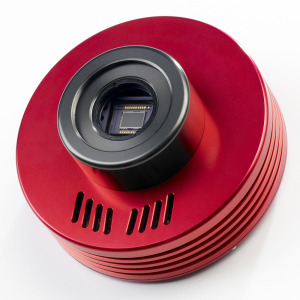
\includegraphics[width=0.7\linewidth]{../images/ccd2}
	\caption[CCD ATIK-314L]{CCD ATIK-314L - \textbf{Fuente:} \cite{Atik364:online} }
	\label{fig:ccd2}
\end{figure} 



La cámara cuenta con un driver INDI, para encargarse del control \cite{atik_indi} de la misma.


\paragraph{Acciones enfoque automático:}

\begin{itemize}
	\item \textbf{Tomar foto:} Solicitar imagen a CCD.
	\item \textbf{Evaluar:} Calcular FWHM imagen.
	\item \textbf{Solicitar nuevo foco:} Mover enfocador en una dirección, un determinado número de pasos.  
\end{itemize}

Con las operaciones anteriores pasamos a definir una serie de algoritmos de autoenfoque cuyo funcionamiento general se muestra en la figura~\ref{fig:op_sis}.

\begin{figure}
	\centering
	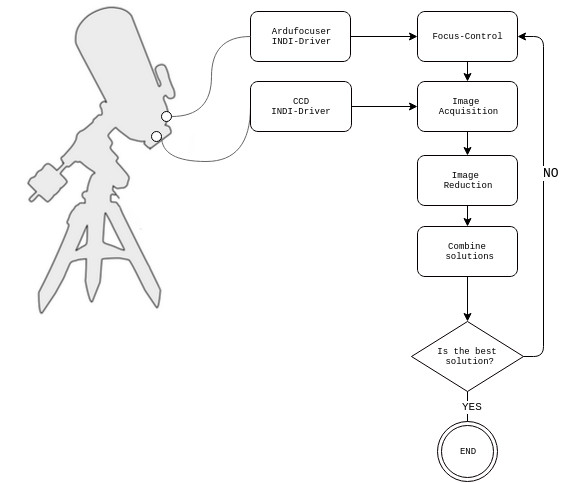
\includegraphics[width=1\linewidth]{../images/procesamiento_imagen}
	\caption[Diagrama operaciones en el sistema]{ Método propuesto }
	\label{fig:op_sis}
\end{figure}


\subsection{Algoritmo búsqueda a ciegas}

Este algoritmo consiste en hacer una primera aproximación rápida del enfoque, buscando la posición adecuada para que pueda funcionar los siguientes algoritmos. Es por ello que se denomina ``a ciegas'' puesto que el sistema no tiene ninguna información del estado anterior. La idea fundamental es que detecte cuando se empiezan a detectar estrellas (figura~\ref{fig:Algoritmo1-Focuser}).

\begin{figure}
\centering
\includegraphics[width=0.9\linewidth]{../images/Algoritmo_ACiegas}
\caption[Algoritmo - A Ciegas]{Algoritmo - A Ciegas}
\label{fig:Algoritmo1-Focuser}
\end{figure}

\begin{lstlisting}[language=python]
INICIO [EnfoqueACiegas]
    Direccion = 0
    NumeroPasos = 1
    FocuserPosition = 0
    FocuserPosition = moverEnfocadorHastaTope(Direccion)
    Direccion = 1
    Imagen = PedirImagenCCD()
    exitenEstrellas = DetectarEstrellas(Imagen)
    WHILE !exitenEstrellas  :
        FocuserPosition=moverEnfocador(Direccion, NumeroPasos)
        Imagen = PedirImagenCCD()
        exitenEstrellas = DetectarEstrellas(Imagen)
        
FIN : return  FocuserPosition    
\end{lstlisting} 



\subsection{Algoritmo autofocus básico}

Con este algoritmo conseguimos llegar al máximo de enfoque (figura~\ref{fig:Algoritmo2-Focuser}).

\begin{figure}[]
	\centering
	\includegraphics[width=0.7\linewidth]{../images/Algoritmo1FINAL}
	\caption[Algoritmo de autofocus básico]{Algoritmo de autofocus básico}
	\label{fig:Algoritmo2-Focuser}
\end{figure}

\begin{lstlisting}[language=python]
INICIO [EnfoqueBase]
    Direccion = 1
    NumeroPasos = 1
    FocuserPosition = 0
    Imagen = PedirImagenCCD()
    fwhm2 = CalcularFwhm(Imagen)
    fwhm1 = 99
    
    WHILE fwhm2 < fwhm1 :
        fwhm1 = fwhm2
        FocuserPosition=moverEnfocador(Direccion, NumeroPasos)
        Imagen = PedirImagenCCD()
        fwhm2 = CalcularFwhm(Imagen)
        
FIN : return  FocuserPosition   
\end{lstlisting} 


\subsection{Algoritmo autofocus para evitar problemas de seeing}

Con este algoritmo conseguimos llegar al máximo de enfoque evitando de manera más eficiente las perturbaciones atmosféricas (figura~\ref{fig:Algoritmo3-Focuser}).

\begin{figure}[]
	\centering
	\includegraphics[width=1\linewidth]{../images/AlgoritmoSeeingFinal}
	\caption[Algoritmo de autofocus (seeing)]{Algoritmo de autofocus para evitar problemas de seeing}
	\label{fig:Algoritmo3-Focuser}
\end{figure}

\begin{lstlisting}[language=python]
DEFINE [TomaFotosYCalcularMediaFWHM()]
    FOR i=0;i<10;i++ :  
        Imagen = PedirImagenCCD()
        SumFwhm += CalcularFwhm(Imagen)
   MeanFwhm = SumFwhm / 10
FIN : return  MeanFwhm

INICIO [EnfoqueSeeing]
    Direccion = 1
    NumeroPasos = 1
    FocuserPosition = 0
    fwhm1 = TomaFotosYCalcularMediaFWHM()
    fwhm2 = 99
    
    WHILE fwhm2 < fwhm1 :
        fwhm2 = fwhm1
        FocuserPosition=moverEnfocador(Direccion, NumeroPasos)
        fwhm2 = TomaFotosYCalcularMediaFWHM()
        
    FIN : return  FocuserPosition   
\end{lstlisting} 





\subsection{Algoritmo autofocus para evitar problemas de backlash}

Con este algoritmo conseguimos llegar al máximo de enfoque evitando problemas de backlash (figura~\ref{fig:Algoritmo4-Focuser}).

\begin{figure}[]
	\centering
	\includegraphics[width=0.8\linewidth]{../images/AlgoritmoBacklashFINAL}
	\caption[Algoritmo de autofocus (backlash)]{Algoritmo de autofocus para evitar problemas de backlash}
	\label{fig:Algoritmo4-Focuser}
\end{figure}

\begin{lstlisting}[language=python]
DEFINE [TomaFotosYCalcularMediaFWHM()]
    FOR i=0;i<10;i++ :  
        Imagen = PedirImagenCCD()
        SumFwhm += CalcularFwhm(Imagen)
   MeanFwhm = SumFwhm / 10
FIN : return  MeanFwhm

INICIO [EnfoqueBacklash]
    Direccion = 1
    NumeroPasos = 1
    FocuserPosition = 0
    fwhm1 = TomaFotosYCalcularMediaFWHM()
    fwhm2 = 99
    
    WHILE fwhm2 < fwhm1 :
        fwhm2 = fwhm1
        FocuserPosition=moverEnfocador(Direccion, NumeroPasos)
        fwhm2 = TomaFotosYCalcularMediaFWHM()
    
    BestFocusPosition=FocuserPosition
    
    FocuserPosition = moverEnfocador(FocuserPosition-10)
    
    FocuserPosition = moverEnfocador(BestFocusPosition)
    
    FIN : return  FocuserPosition   
\end{lstlisting} 


\section{Métodos de simulación}

Aquí se muestra una breve introducción al simulador que se ha diseñado para poder realizar pruebas de enfoque sin tener que usar instrumental en directo ya que realizar la implementación y pruebas en vivo puede llegar a ser tedioso, dado que requiere unas condiciones de observación muy específicas. 

Es por ello que se opta por implementar un simulador de CCD y Enfocador. 

Este software cuenta con las mismas funciones que el sistema real (tomar foto, avanza enfocador, retrocede), pero se ejecuta en un entorno virtual. 

Además para asegurar que es fiel a la realidad, su estado inicial debe ser aleatorio.

